\section{Is Decodability Enough? Rethinking Concept-Level Control in Medical Vision-Language Models}\label{sec:raw}
\subsection{From readable features to controlled answers}
A concept can be extracted from a medical VLM's representations without controlling its answers. RAW (Read--Answer--Write)~\citep{raw} separates these properties through read, answer, and write tests. Hanqi Jiang is first author; Lei Xing is corresponding author. A concept is \emph{readable} if a probe beats its controls. It is \emph{answerable} if answer AUROC exceeds 0.5. It is \emph{owned} if writing its own probe direction into consumed visual tokens moves its own answer more than random and sham controls and all five competing-concept directions. The ownership test is consequently stronger than merely observing an answer shift after an intervention.
Figure~\ref{fig:raw_framework} illustrates the read and write tests.
\begin{figure}[!t]\centering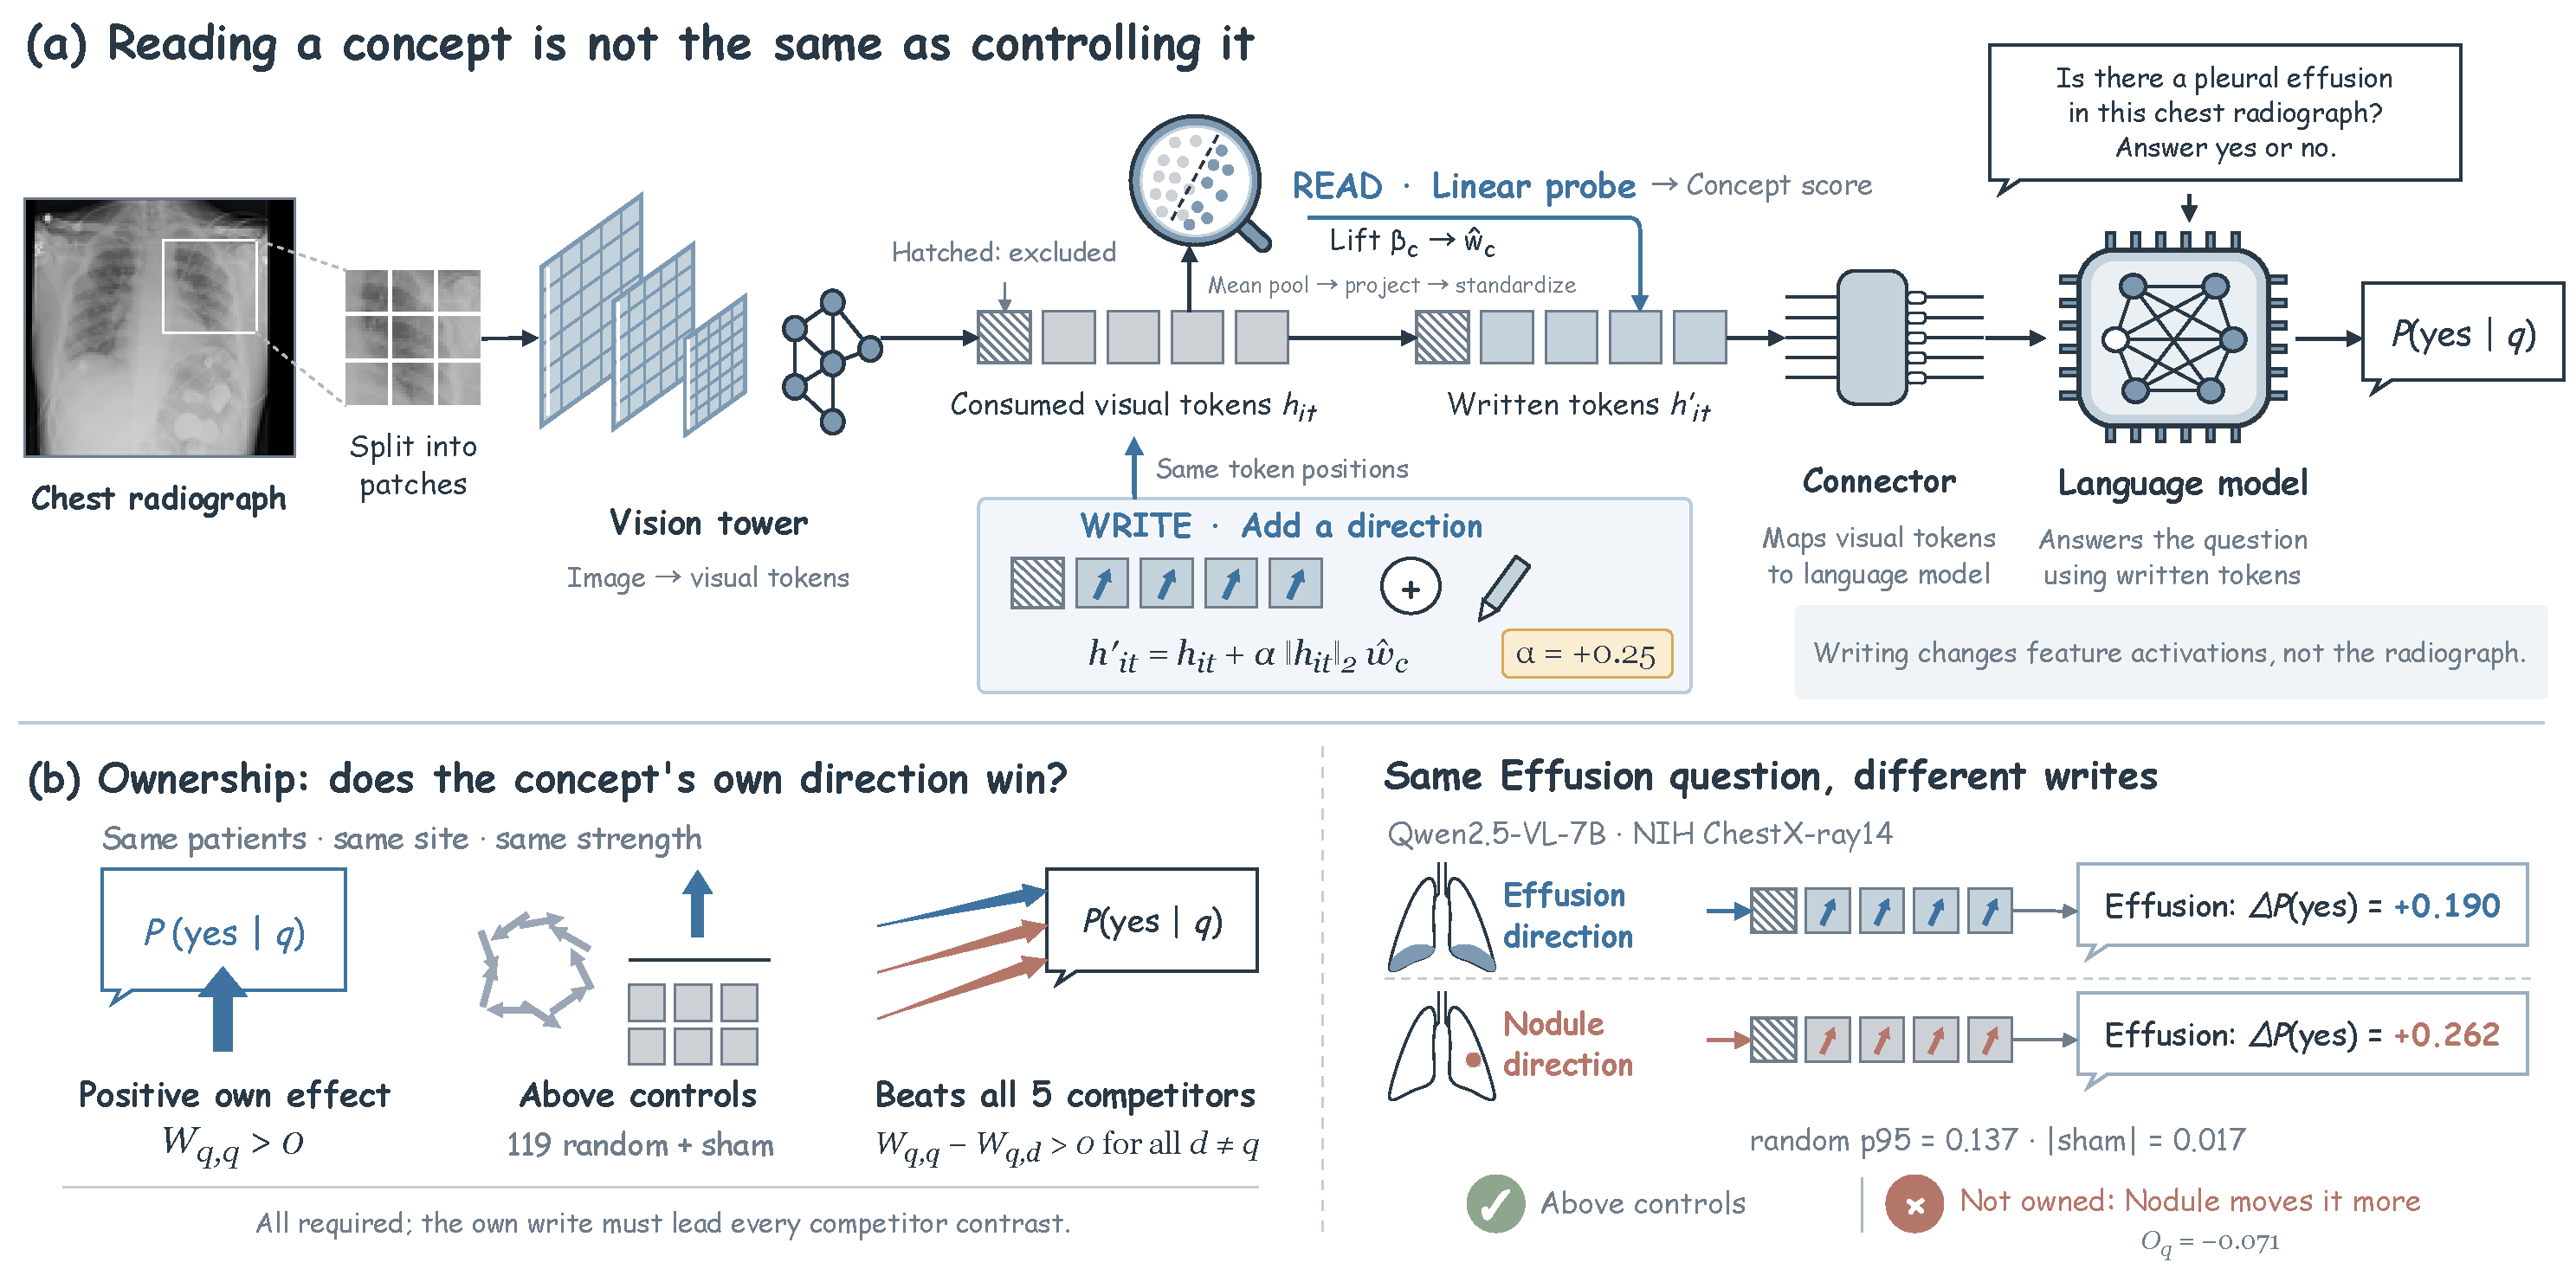
\includegraphics[width=\textwidth,height=.30\textheight,keepaspectratio]{figures/raw_framework.pdf}\caption{RAW reads a concept with a probe applied to pooled visual tokens at a selected vision layer. The probe coefficients yield a lifted write direction that is added to the consumed tokens; the connector and language model then produce the answer probability. Writes along different directions form a matrix of answer-probability changes. The ownership margin compares the change from a question's own direction with the strongest competing direction. An answer direction provides another control for the read and write analysis. Adapted from RAW Fig. 2. Source: RAW~\citep{raw}.}\label{fig:raw_framework}\end{figure}

The study examines 25 checkpoints across 12 families, ranging from 3B to 72B, using NIH ChestX-ray14 and CheXpert Plus with COCO as a control. The campaign comprises 450 cells, approximately 30 million answers, and approximately 3,000 A100-hours. For chest findings, 85\% are readable and 86\% answerable, but only 15\% are owned, compared with 78\% ownership for COCO.

Checkpoints sharing a visual tower can differ, implicating the connector and language model in the deficit. An answer-fitted direction is owned more often and is nearly orthogonal to the probe direction, with cosine 0.18. Thus the direction best suited to reading a concept need not be the direction that most effectively changes generation. This observation also motivates the survey's call to investigate components beyond the image encoder.

\subsection{Scope and role in the dissertation}
The analysis is limited to open-weight systems, chest radiographs, and rank-one writes at two sites. The intervention cannot resolve all forms of distributed or nonlinear use. RAW is a diagnostic contribution, not an efficiency-centered one: its substantial experimental cost should not be described as a resource saving. Its role is to motivate the transition from representations that may encode evidence to methods that make an answer's relationship to localized evidence inspectable.
